\documentclass{jfp}

\usepackage{ifpdf}
\usepackage{ifthen}
\usepackage{subfigure}
\usepackage{epsfig}

\title{\LARGE \bf
A simpler approach to waterfall
}
\author{Chris Nicholls, Irina Voiculescu and Stuart Golodetz
}
%\institute{Oxford University Computing Laboratory}

\begin{document}

\maketitle
\pagestyle{empty}

\begin{abstract}
It is useful to be able to identify particular features in a set of
images automatically. One application is in the treatment of cancer,
where algorithms can be used to aid the detection and classification
of organ and tumour tissue. This is the main motivation for this
project, although the algorithm presented is a generic one, with many
applications. SAY SOMETHING ABOUT FP APPROACH
\end{abstract}

\section{Introduction}

@@@

 - segmentation is ...

 - waterfall algorithm for segmentation

 - existing implementation (arguably overly complicated)

 - we have a better, simpler one

 - we will illustrate it on CT scans


\section{Motivation}

 This project is motivated by the need to {\em segment\/} greyscale
 images originating from computerised tomography (CT) scanners. That
 is, we would like to fit contours around organ tissue featured in
 each image. A pair of algorithms called the watershed and waterfall
 algorithms have been shown to be effective for this
 purpose~\cite{golodetz}, although other approaches exist. This paper
 presents a new, simplified, implementation of the {\em waterfall\/}
 algorithm.

\section{Conventional imperative approach to waterfall}

 - it is `very imperative'

 - construct MST and consume it from any side

 - include refs

 - high-level description of waterfall (space permitting)



The watershed algorithm, introduced by Beucher and
Lantuejoul~\cite{beucher79}, produces a segmentation of an image,
grouping together regions of pixels deemed to be similar. Usually,
`similar' refers to similarity in the greyscale values, though other
approaches are possible. A typical problem of the watershed algorithm
is that it over-segments images significantly, leading to far more
regions than can be handled sensibly, as illustrated in
Figure~\ref{fig:oversegmented}.

%---
%---
\begin{figure}
\centering
\ifpdf
        \subfigure{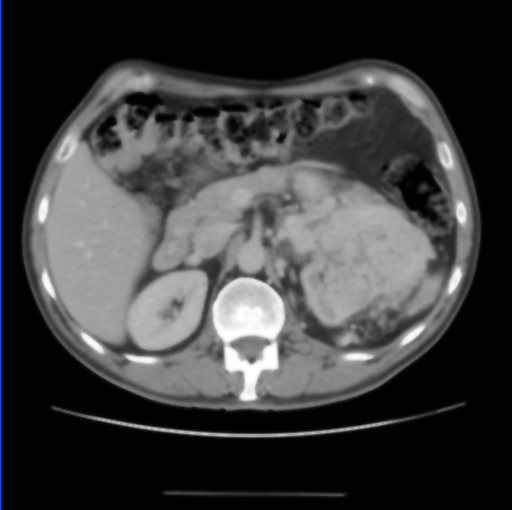
\epsfig{file=image0.png, width=.240\linewidth}}%
        \hspace{1mm}%
        \subfigure{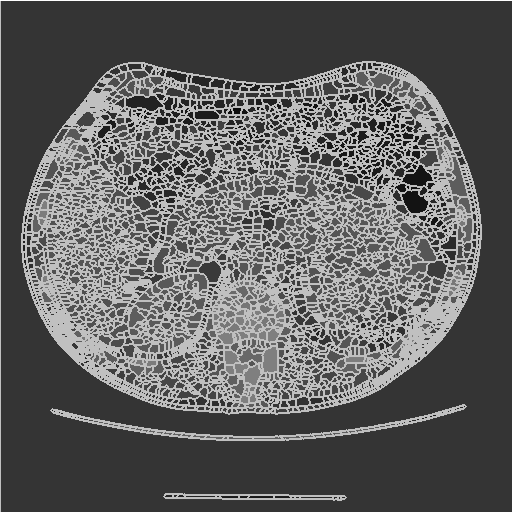
\epsfig{file=image5.png, width=.240\linewidth}}%
\else
        % TODO
\fi
\caption{Example of over-segmentation, output by applying the watershed
  algorithm to an axial slice of a CT volume. The individual regions
  are small and do not correspond to any anatomic features.}
\label{fig:oversegmented}
\end{figure}
%---
%\vspace{-5mm}
%
The waterfall algorithm~\cite{beucher94,marcotegui} is an iterative process which can extract
further structure from an initial watershed segmentation. The
waterfall yields a partition forest hierarchy, which is a
comprehensive data structure which  can subsequently be used  for
feature identification.  Figure~\ref{fig:waterfall} illustrates the
various layers that result from applying the waterfall algorithm to
the segmentation shown in Figure~\ref{fig:oversegmented}.  Each
iteration of the algorithm yields a higher-level grouping of the
regions in the previous layer.
%\vspace{-5mm}
%---
\begin{figure}
\centering
\ifpdf
%        \subfigure{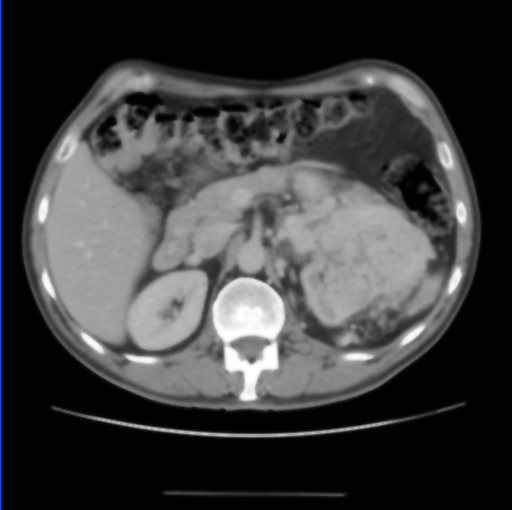
\epsfig{file=image0.png, height=.175\linewidth}}%
%        \hspace{4mm}%
%        \subfigure{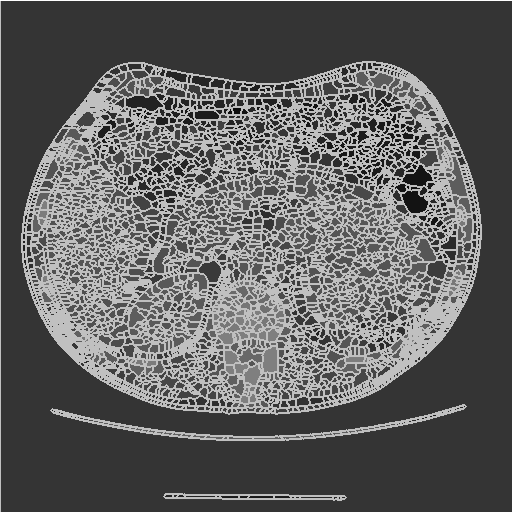
\epsfig{file=image5.png, width=.240\linewidth}}%
%        \hspace{1mm}%
        \subfigure{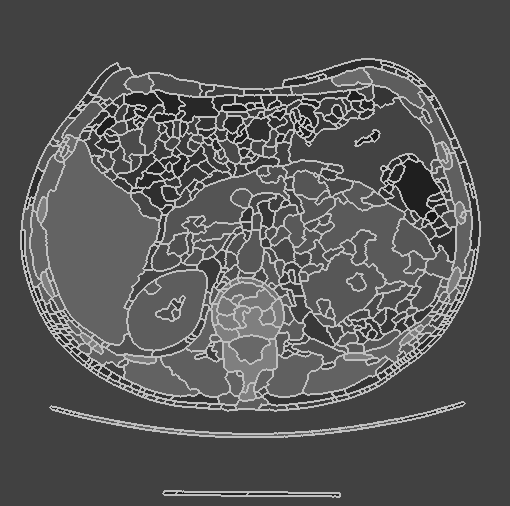
\epsfig{file=image4.png, width=.260\linewidth}}%
        \hspace{1mm}%
        \subfigure{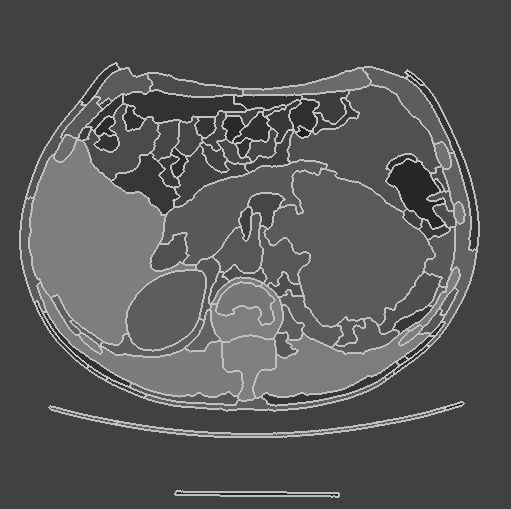
\epsfig{file=image2.png, width=.260\linewidth}}%
        \hspace{1mm}%
        \subfigure{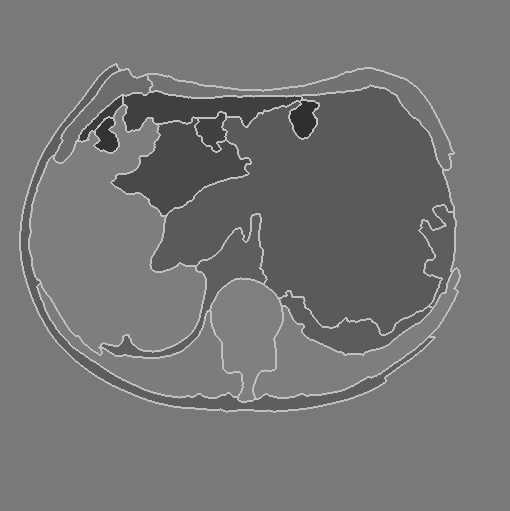
\epsfig{file=image1.png, width=.260\linewidth}}%
\else
        % TODO
\fi
\caption{Hierarchy of segmentations produced by applying the waterfall
  algorithm to the output of the watershed illustrated in
  Figure~\ref{fig:oversegmented}, showing regions merging successively
  (left to right).}
\label{fig:waterfall}
\end{figure}
%---

Both the watershed and the waterfall algorithms are based on a
geographical metaphor. The image is regarded as a landscape, with each
grey value at representing the height of the terrain at given $(x,y)$
coordinates.
% being proportional to the terrain height.
%
The valleys are
in the darker areas, whereas the lighter areas are regarded as peaks.

The waterfall algorithm can then be imagined
as a flooding process. The water falls into (low) catchment basins and
gradually fills them up to the nearest boundaries, sometimes spilling
into adjacent regions. This process continues until the whole image
becomes a single basin. The intermediate stages of the process can be
regarded as intermediate segmentations of the image, with each basin
representing a region.

An implementation of this algorithm, proposed by Marcotegui and
Beucher~\cite{marcotegui}, involves the construction of a Minimum
Spanning Tree (MST) and the gradual elision of some of its edges.  Its
nodes are initially the regions of the watershed output and its edges
are the lowest pass points on the boundaries between these regions;
the nodes and edges in subsequent layers are derived from these
initial ones through a merging process.

A regional minimum edge of a graph $G$ is part of a connected subgraph
of $G$ whose edges have the same weight as each other, and whose
adjacent edges in $G$ have strictly higher weights. The waterfall
algorithm relies heavily on finding these regional minimum edges,
eliding them and rebuilding the MST -- a process which not only
requires careful implementation of the MST but, crucially, is
relatively complex and hard to implement.

\iffalse
The collection of regional minimum edges of a graph $G$ is a connected
subgraph of $G$ whose edges have the same weight as each other, and
whose adjacent edges in $G$ have strictly higher weights. The
waterfall algorithm relies heavily on finding these regional minimum
edges, eliding them and rebuilding the MST -- a process which not only
requires careful implementation of the MST but, more importantly, is
relatively complex and hard to implement.
\fi


\section{Functional approach to waterfall}

 - single recursive pass (fairly opaque but no special cases for the
 detail)


In this paper we present a new data structure for the waterfall
algorithm that simplifies the process and improves efficiency compared
to current implementations. It is based on a recursive-tree data
structure and a recursive relation on the nodes rather than the
conventional iterative transformations.


\subsection{How it works}

 MST (only briefly)

\begin{verbatim}
 Eliding edges - cases I to IV

 Case I     parent -> child ->

   Recurse on child first, as there's bound to be a minimum further
   down, then combine parent with the result of that operation.

 Case II    parent <-> child

   Can't just elide the edge between parent and child and merge the
   two into one node, because there may be other children of the
   parent which need to be recursed on separately from the children of
   the child. (NB Illustrate this on the sample tree.)  Well, after
   further discussion it seems that we could, in fact, just elide that
   edge, but we want to think about it more.
   
   Use the recurseWithNoDownMerging function, which recurses without
   looking for a minimum first. (Children can merge up with the
   current node, but the current node does not attempt to merge down
   with its children.)

 Case III   parent -> ? (where '?' can be above or below the parent)
            |
            child ->

   This is similar to Case I. After recursing there is no need to
   combine the parent with the result of the recursion on the
   child. Simply keep in place the edge between the parent and child.

 Case IV    parent -> ? (where '?' can be above or below the parent)
            ^
            |
            child

    Use the recurseWithNodownMerging but do combine the result
    afterwards, as in Case II. (This is semantically identical to Case
    II but is treated separately for clarity of cases considered.)


[In the actual paper, consider cases II and III swapped, and explain
that it's more important what the child "wants" than what the parent
"wants". No, scrap that.]

Then for each parent iterate through each child...
\end{verbatim}

\subsection{Correctness?}

(note that there is arbitrary choice about edges of same weight)


\section{Results}


\section{Conclusions}

 - can be done in pure FP style

 - clearer to write/code

 - shorter code and simpler data structures


The main advantage of our approach to the waterfall problem is that
the algorithm uses a single loop to walk the MST and is therefore
simpler to implement. For each iteration, it walks the MST bottom-up
in a single pass and merges regions that belong together. The
waterfall algorithm, thus improved, produces the same layers of
segmented images, combined in a hierarchical structure that can be
processed for feature identification.

A further advantage of our approach is that the algorithm can can be
written in pure functional style. In particular, we have implemented
it in Haskell. For this reason, the memory requirements are not
directly comparable to existing imperative implementations, but we are
about to integrate this new approach into an existing C++ code base.

We are also in the process of constructing a formal proof of
correctness, which we hope to present at a later date. We have tested
both algorithms on a number of small, measurable test cases and found
that they produce the same output. Empirical tests indicate that this
is also true of larger test cases, such as axial slices of CT volumes.

Production of partition forests in this manner is independent of this
application and has many applications outside of the field of medical
imaging.

\bibstyle{plain}

\begin{thebibliography}{2}
 	

\bibitem{golodetz}{Stuart Golodetz, Irina Voiculescu and Stephen
  Cameron.  {\em Region Analysis of Abdominal CT Scans using Image
    Partition Forests}. In Proceedings of CSTST 2008 pages
  432-7. October 2008.}

\bibitem{beucher79}{S.\ Beucher, C.\ Lantuejoul. {\em Use of
    watersheds in contour detection}. International Workshop on image
  processing, real-time edge and motion detection/estimation, Rennes,
  France, Sept.\ 1979.}

\bibitem{beucher94}{Serge Beucher. {\em Watershed, hierarchical
    segmentation and waterfall algorithm}. In Mathematical Morphology
  and its Applications to Image Processing, Proc.\ ISMM 94, pages
  69-76, Fontainebleau, France, 1994. Kluwer Ac.\ Publ.}

\bibitem{marcotegui}{Beatriz Marcotegui and Serge Beucher, {\em Fast
    Implementation of Waterfall Based on Graphs}. In Mathematical
  Morphology: 40 Years On, Springer Netherlands, 2005.}

\end{thebibliography}

\end{document}

